\documentclass{article}
\usepackage[utf8]{inputenc}
\usepackage[spanish]{babel}
\usepackage{listings}
\usepackage{graphicx}
\graphicspath{ {images/} }
\usepackage{cite}


\begin{document}
\begin{titlepage}
    \begin{center}
        \vspace*{1cm} 
            
        \Huge
        \textbf{Implementación}
            
        \vspace{0.5cm}
        \LARGE
        Informe 
            
        \vspace{1.5cm}
            
        \textbf{Jhonny Alejandro Ortiz Osorio}
        
        \textbf{C.C: 1001015092}
        
        \vfill
            
        \vspace{0.8cm}
            
        \Large
        Departamento de Ingeniería Electrónica y Telecomunicaciones\\
        Universidad de Antioquia\\
        Medellín\\
        Septiembre de 2021
            
    \end{center}
\end{titlepage}


\tableofcontents
\newpage
\section{Clases Implementadas}\label{intro}
En la solución del problema se utilizaron en total 4 clases: 

\subsection{QImage}
Es una clase establecida de Qt que nos permite manejar imágenes. Tiene métodos que nos permite leer una imagen, escalar el tamaño de una imagen o sacar información de los colores de cada pixel. En este caso solo se utilizó el método de leer imágenes y el método pixelcolor para sacar el color de un pixel en formato RGB.

\subsection{Adafruit NeoPixel}
Es una clase establecida de Arduino que nos permite controlar tiras de neopixel. De esta clase se utilizó el método setPixelColor que nos permite darle un color a un pixel en el formato de color RGB.

\subsection{Escalamiento}
Es una clase propia que permite procesar una imagen y ajustarla a un tamaño determinado. Esta clase el submuestreo y sobremuestreo de imágenes para poder procesar la imagen apropiadamente.

\subsection{Escritura}
Es una clase propia que escribe en un archivo de texto una información dada.

\newpage
\section{Estructura de las clases}\label{intro}
\subsection{Clase Escalamiento}
\begin{figure}[h]
    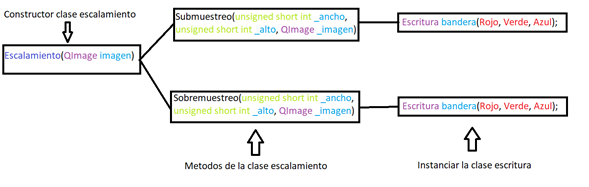
\includegraphics[width=15cm]{image1.png}
    \centering
    \caption{Estructura Clase Escalamiento}
    \label{fig:image1}
    \vspace{1.5cm}
    \end{figure}

\subsection{Clase Escritura}
\begin{figure}[h]
    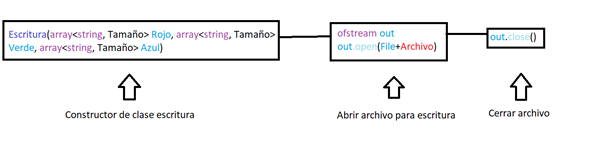
\includegraphics[width=15cm]{image2.png}
    \centering
    \caption{Estructura Clase Escritura}
    \label{fig:image}
    \vspace{1.5cm}
    \end{figure}

\newpage    
\section{Módulos de código}\label{intro}
En la primera parte del programa instanciamos la clase QImage para poder sacar toda la información de la imagen que se va a procesar. Después, se instancia la clase Escalamiento, entregando como parámetro al constructor el objeto QImage que se creó anteriormente, en la clase Escalamiento se procesa la imagen con el método de submuestreo o sobremuestreo, esto depende del tamaño de la imagen, por ultimo se instancia la clase Escritura dentro del constructor de la clase Escalamiento para poder escribir en un archivo toda la información de la imagen ya procesada.

\section{Circuito}\label{intro}
\subsection{Elementos Utilizados}
    \begin{figure}[h]
    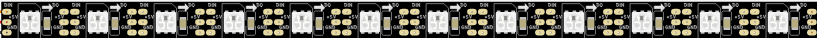
\includegraphics[width=10cm]{NeoPixel.png}
    \centering
    \caption{Tiras de NeoPixel}
    \label{fig:image}
    \vspace{1.5cm}
    \end{figure}

    \begin{figure}[h]
    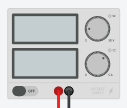
\includegraphics[width=5cm]{SuministroEnergia.png}
    \centering
    \caption{Suministro de Energia}
    \label{fig:image}
    \vspace{1.5cm}
    \end{figure}
    
    \begin{figure}[h]
    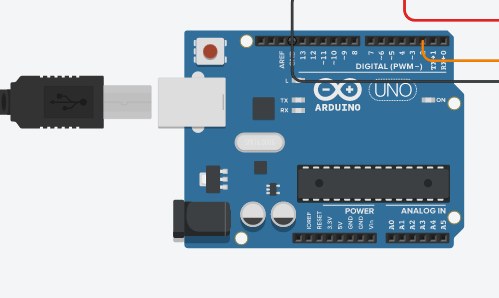
\includegraphics[width=7cm]{Arduino.png}
    \centering
    \caption{Arduino Uno}
    \label{fig:image}
    \vspace{1.5cm}
    \end{figure}
\newpage
\subsection{Circuito Completo}
Para conectar todo el circuito se necesitaron 12 tiras de neopixeles, un Arduino y un suministro de energía. Se conecta el suministro de energía con un acople de tierras y la parte positiva se conecta al positivo de la primera tira de neopixeles, después de conectan todas las tierras y positivos de las tiras de neopixeles faltantes. El siguiente paso es conectar un pin digital del Arduino a la entrada de la primera tira de neopixeles y la salida de esta tira se conecta a la entrada de la siguiente tira de neopixeles.

    \begin{figure}[h]
    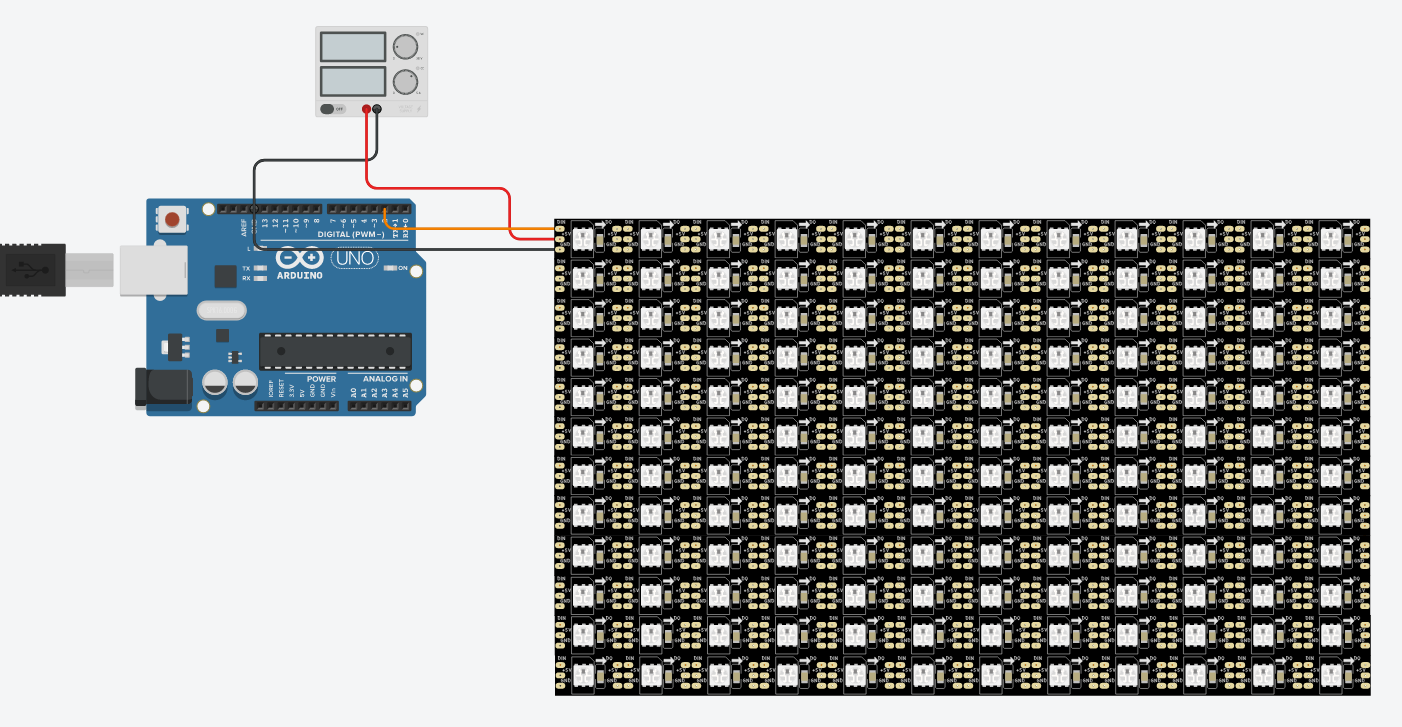
\includegraphics[width=10cm]{Circuito.png}
    \centering
    \caption{Circuito}
    \label{fig:image}
    \vspace{1.5cm}
    \end{figure}
\end{document}